\chapter{Implementation}\label{ch:Implementation}

\section{Exploratory Data Analysis}
All code for the EDA detailed in this chapter can be found at:\newline https://github.com/AMacleod79/HonoursProjectCode
\subsection{Data Overview}

A total of eight health related datasets were chosen to examine the problem of class imbalance. As previously detailed in chapter 3, these datasets were publicly available on kaggle.com and having already been processed to some extent to either anonymise the data or render the data more workable.\newline
The extent of class imbalance varied across the different datasets and for some the imbalance was not very severe at all. In some cases a modified version of the dataset was created to attempt to replicate the real-life prevalence of the disease.\newline

\subsubsection{Cervical cancer dataset}
The cervical cancer dataset was obtained from kaggle.com. \newline
(see https://www.kaggle.com/loveall/cervical-cancer-risk-classification)\newline
This dataset looks at predicting cervical cancer diagnostic based on well known risk factors. Cervical cancer is a complicated diagnostic to make and as such there is not one single test to confirm diagnostic. A diagnostic column was created as an average from the four possible diagnostic test used  (last four column: Hinselmann, Schiller, Citology, Biopsy ) \citep{Fernandes:2017td, Wu:2017fa}.\newline
The dataset contains 858 instances with 32 features and 4 target variables for each of the test carried out.
The exploratory data analysis carried out on this dataset can be found in the cited github repository as CervicalCancerEDA.R.
The 32 features focus on lifestyle factors previously shown to influence cervical cancer risk in women, namely:
\begin{itemize}
    \item Age
    \item Number of sexual partners
    \item First sexual intercourse (age)
    \item Num of pregnancies
    \item Smokes (boolean)
    \item Smokes (years)
    \item Smokes (packs/year)
    \item Hormonal Contraceptives (boolean)
    \item Hormonal Contraceptives (years)
    \item IUD (boolean)
    \item IUD (years)
    \item STDs (boolean)
    \item STDs (number)
    \item STDs:condylomatosis (boolean)
    \item STDs:cervical condylomatosis (boolean)
    \item STDs:vaginal condylomatosis (boolean)
    \item STDs:vulvo-perineal condylomatosis (boolean)
    \item STDs:syphilis (boolean)
    \item STDs:pelvic inflammatory disease (boolean)
    \item STDs:genital herpes (boolean)
    \item STDs:molluscum contagiosum (boolean)
    \item STDs:AIDS (boolean)
    \item STDs:HIV (boolean)
    \item STDs:Hepatitis B (boolean)
    \item STDs:HPV (boolean)
    \item STDs: Number of diagnosis
    \item STDs: Time since first diagnosis
    \item STDs: Time since last diagnosis
    \item Dx:Cancer (previous diagnostic of cervical cancer)
    \item Dx:CIN (previous diagnostic of cervical intreaepithelial neoplasia)
    \item Dx:HPV (previous diagnostic of HPV)
    \item Dx (previous diagnostic of cervical cancer)
    \item Hinselmann (target variable)
    \item Schiller (target variable)
    \item Citology (target variable)
    \item Biopsy (target variable)
\end{itemize}

The exact meaning of each variable was not always straight forward to understand as the data was uploaded to kaggle by someone else than the original authors. The UCI repository also gives access to the data with scant details on the meaning of each column. The original work by Fernandes and colleagues \citep{Fernandes:2017td} does not clearly define each of the column and the link to the dataset from the published article now returns a 404 error. With these considerations in mind and based on other work carried out by other authors (Wu and colleagues \citep{Wu:2017fa}), the above attributes were used and a composite target variable was created (see below).\newline
An examination of the data structure showed that 27 columns were factors, with the column "smoke pack per year" showing 63 levels. The Random Forest function in R will only handle a maximum of 53 levels and therefore the data in this column needed to be manipulated to accommodate this restriction. \newline
First any missing values was replaced by the mean for the column. Next, it was found that there were a high number of discrete values between 0 and 1 for the number of pack of cigarettes smoked per year, and these were all considered as independent levels. All values that were less than 1 for this column were replaced by 0, taking the total number of levels for the column from 63 to 42, which is now manageable by Random Forest.\newline
All the other columns had a number of factor levels smaller than 53 and were left as such, however any missing value was replaced by the mean for the column in which it was found.\newline
A composite target variable calculated as a mean value of all 4 target variables (Hinselmann, Schiller, Citology, Biopsy was created and added as the last column in the dataset (rounded to 0 or 1).\newline
The pre-processed dataset was exported as a new .csv file to be used in the experimental stages of this projects (see table 4.2).
Finally the class distribution was represented as a bar chart and detailed in a table (see Figure 4.1 and table 4.3) 

\subsubsection{Breast cancer dataset}
The Breast Cancer dataset was obtained from kaggle.com. \newline
(see https://www.kaggle.com/uciml/breast-cancer-wisconsin-data) \newline
This dataset was developed with a view to train and test algorithms to determine whether a breast tumour was malignant or benign \citep{OLMangasarian:1994ue}. \newline
There are  569 instances each with 32 attributes and one target label (B for benign and M for malignant).\newline
The attributes were computed from images of a fine needle aspirate of a breast mass to describe the characteristics of the cell nuclei present in the image. The features were as follows:
\begin{itemize}
    \item radius (mean of distances from center to points on the perimeter)
    \item texture (standard deviation of gray-scale values) 
    \item perimeter 
    \item area 
    \item smoothness (local variation in radius lengths) 
    \item compactness (perimeter\^2 / area - 1.0)
    \item concavity (severity of concave portions of the contour)
    \item concave points (number of concave portions of the contour)
    \item symmetry
    \item fractal dimension ("coastline approximation" - 1)
\end{itemize}
The mean, standard error and mean of of three largest values (i.e. the "worst") for each of the feature was calculated and documented as a feature for each image.\newline

The exploratory data analysis carried out on this dataset is documented in the cited github repository as BreastCancerEDA.R.\newline
An analysis of the data structure showed no missing values. The target variable was expressed as B or M and was recoded to be either 0 (benign) or 1 (malignant), further the target variable was originally the second column but for ease of analysis in the next stages of the project this was moved to be the last column and renamed "Label".\newline
The modified dataset was exported as a .csv file for later use in the project (see table 4.2).\newline
Finally the class distribution of the dataset was computed and is shown in figure 4.1 with details shown in table 4.3.\newline 


\subsubsection{Liver Disease dataset}
This dataset was obtained from kaggle.com.\newline
(see https://www.kaggle.com/jeevannagaraj/indian-liver-patient-dataset). \newline
There are 583 instances of patient records with 10 attributes and one target variable to determine whether the patient is a liver patient or not \citep{Ramana:2011tn}. The attributes are various biochemical measures of liver health as well as patient specific information such as age and gender:
\begin{itemize}
    \item Age of patient
    \item Gender of patient
    \item Total Bilirubin
    \item Direct Bilirubin
    \item Alkaline Phosphatase
    \item Alamine Amino-transferase (sgpt)
    \item Aspartate Amino-transferase (sgot)
    \item Total Proteins
    \item Albumin
    \item Albumin and Globulin Ratio
    \item is patient (target label)
\end{itemize}

The exploratory data analysis carried out on this dataset is documented in the cited github repository as LiverDataEDA.R.\newline
The target label was set to 1 (not a liver patient) and 2 (liver patient), for consistency with respect to the other datasets used in this project, the data was recoded to 0 (not a liver patient) and 1 (liver patient).\newline
A check for missing data revealed only four instances missing a value in the albumin and globulin ratio. The missing values were replaced with the mean for that column.\newline
The pre-processed dataset was exported as a .csv file for later use in the project (see table 4.2).\newline
The class distribution was compiled and presented as a graph (see figure 4.1) and the details of the class distribution were shown in table 4.3.\newline


\subsubsection{Diabetes}
This dataset was obtained from kaggle.com:\newline
( see https://www.kaggle.com/uciml/pima-indians-diabetes-database)\newline
There are 768 instances of health data from female Pima Indian patients of at least 21 years of age. There are 8 attributes and one target variable. The target variable indicates whether the individual will develop diabetes within 5 years (1) or not (0). The attributes were as follows:
\begin{itemize}
    \item Pregnancies indicates the number of times the patient pregnant
    \item GlucosePlasma indicates the glucose concentration at 2 hours in an oral glucose tolerance test
    \item BloodPressureDiastolic indicates the diastolic blood pressure (mm Hg)
    \item SkinThicknessTriceps indicates triceps skin fold thickness ( in mm)
    \item Insulin2-Hour indicates the serum insulin concentration  (mu U/ml)
    \item BMI indicates body mass index (weight in kg/(height in m \textsuperscript{2})
    \item DiabetesPedigreeFunctionDiabetes is a pedigree function calculated by the original authors of the study which takes family history of diabeted into account
    \item Age records the age of the patient (years)
\end{itemize}
 The dataset was used in a study looking at the ADAP algorithm and further details about the pedigree function and other variables can be found in the article \citep{Smith:1988wy}.
 
The exploratory data analysis carried out on this dataset is documented in the cited github repository as DiabetesEDA.R.\newline
The target label was already set to 0 (did not develop diabetes within 5 years) and 1 (did develop diabetes within 5 years), so no recoding of the data was necessary.\newline
A check for missing data revealed none, and Smith \textit{et al.,} indicate that they replaced any missing data with 0 (which does not always make sense, e.g. for blood pressure). No further modification of the dataset were necessary and the pre-processed dataset was saved as .csv file for later use (see table 4.2).
The class distribution was compiled and presented as a graph (see figure 4.1) and details of the class distribution can be seen in table 4.3. 

\subsubsection{Lower Back Pain dataset}

This dataset was originally built by Dr Henrique da Mota with a view to classify patient as one of 3 class: Normal, patients with disk hernia and patients with spondylolisthesis \citep{RochaNeto:2009wp}. In a second classifying task, the two types of sufferers were grouped as one abnormal category. This dataset was first uploaded to UCI (see http://archive.ics.uci.edu/ml/datasets/vertebral+column) and then uploaded to Kaggle (see https://www.kaggle.com/sammy123/lower-back-pain-symptoms-dataset) as a binary classification task dataset (normal/abnormal).\newline
The dataset consists of 310 instances with 13 attributes (12 numeric predictors and 1 target label) as follows:
\begin{itemize}
    \item pelvic incidence
    \item pelvic tilt
    \item lumbar lordosis angle
    \item sacral slope
    \item pelvic radius
    \item degree spondylolisthesis
    \item pelvic slope
    \item Direct tilt
    \item thoracic slope
    \item cervical tilt
    \item sacrum angle
    \item scoliosis slope
\end{itemize}

The exploratory data analysis for this dataset is documented in the cited github repository as LowBackPainEDA.R.\newline
For ease of reading and  manipulation, the columns names were replaced by the actual name of the predictor (removing col x from the name) and the unused column X was removed.\newline
The target label was set as abnormal or normal so the data was recoded to be 1 for abnormal and 0 for normal, in line with the other datasets. There were no missing values in the dataset.\newline
Uncharacteristically for a classification task, the abnormal class contains a higher number of instances than the normal class (see figure 4.1 and table 4.3). This is unusual and in order to observe a class distribution more in line with those seen in other datasets in this project, random sampling of the dataset was  carried out so as to create a modified dataset with more normal samples than abnormal. \newline
To obtain the new dataset, 7\% of the abnormal instances were  retained (resulting in a higher prevalence than current estimates of 1-3\% of low back pain sufferer, \citep{Jordan:2009vx}) and 100 \% of the normal instances were retained. The pre-processed datasets were saved as .csv files for later use (see table 4.2). The new class distribution is also shown on figure 4.1 with details outlined in table 4.3.\newline

\subsubsection{Heart Attack Dataset}
This dataset is a subset from a multi-centre, larger study which looked at patients with and without heart disease. The dataset was obtained from kaggle.\newline 
(see https://www.kaggle.com/imnikhilanand/heart-attack-prediction) \newline
The complete dataset appears to be available from UCI:\newline
https://archive.ics.uci.edu/ml/datasets/heart+Disease \newline 
though some of the files may be corrupted and the classification tasks of the original datasets is not binary.
The original dataset was made up of 76 predictors but in this dataset this has been reduced to 13 and a target variable:
\begin{itemize}
    \item age (in years)
    \item sex (1 = male, 0 = female) 
    \item cp (chest pain type 1-4)
    \item trestbps (resting blood pressure)
    \item chol (serum cholesterol in mg/dl) 
    \item fbs (fasting blood sugar >120 mg/dl, 1= true, 0 =false) 
    \item restecg (resting ECG results - 0 = normal, 1 = ST-T abnormal, 2 = hypertrophy)
    \item thalach (maximum heart rate achieved)
    \item exang (exercise induced angina 1 = yes, 0 = no)
    \item oldpeak (ST depression induced by exercise)
    \item slope (slope of peak exercise ST segment)
    \item ca (number of major vessels coloured fluoroscopy (0-3) 
    \item thal (3 = normal, 6 = fixed defect, 7 = reversable defect) 
\end{itemize}

The exploratory data analysis is documented in the cited github repository as HeartAttackEDA.R.\newline
Nine column contained missing values, and those were replaced with the mean value for that column. Examination of the data structure revealed that columns "chol" (for cholesterol value) and "thalach" (maximum heart rate achieved) were factors with more than 53 levels (the maximum that can be handled by Random Forest), 154 and 72 levels, respectively. The number of levels was reduced by grouping levels into categories, as shown in table 4.1:
\begin{table}[!htbp]
\centering
\begin{tabular}{*5c}
  \hline
  \rowcolor{LightCyan}
  \multicolumn{2}{c}{Cholesterol} & \multicolumn{2}{c}{Thalach} \\
  \hline
  \hline
Level Value & New Level & Level Value & New Level\\ 
  \hline
    $<$100  & 100 & $\leq$90 & 90 \\ 
   $<$175 $\leq$150 & 175 & $>$90 $\leq$95   &  95 \\ 
  $<$200 $\geq$175 & 200 & $>$95 $\leq$100  & 100  \\ 
   $>$200 $\leq$225 & 225 & $>$100 $\leq$105 & 105  \\ 
   $>$225 $<$250  & 250 & $>$105 $\leq$110 & 110  \\ 
   $>$250 $<$275  & 275 & $>$110 $\leq$115 & 115  \\ 
   $>$275 $<$300  & 300 & $>$115 $\leq$120 & 120   \\ 
   $>$300 $<$325  & 325 & $>$120 $\leq$125 & 125   \\ 
   $>$325 $<$350  & 350 & $>$125 $\leq$130 & 130  \\ 
   $>$350 $<$375  & 375 & $>$130 $\leq$135 & 135  \\ 
   $>$375 $<$400  & 400 & $>$135 $\leq$140 & 140 \\ 
   $>$400 $<$425  & 425 & $>$140 $\leq$145 & 145\\ 
   $>$425 $<$450  & 450 & $>$145 $\leq$150 & 150\\ 
   $>$450 $<$475  & 475 & $>$150 $\leq$155 & 155\\ 
   $>$475 $<$500  & 500 & $>$155 $\leq$160 & 160\\ 
  `$>$500 $<$525  & 525 & $>$160 $\leq$165 & 165 \\ 
   $>$525 $<$550  & 550 & $>$165 $\leq$170 & 170 \\ 
   $>$550 $<$575  & 575 & $>$170 $\leq$175 & 175 \\ 
   $>$575 $<$600  & 600 & $>$175 $\leq$180 & 180 \\ 
                  &     & $>$180 $\leq$185 & 185 \\ 
                  &     & $>$185 $\leq$190 & 190 \\ 
   \hline
\end{tabular}
\caption{Grouping of levels for columns "chol" and "thalach" (Heart Disease Dataset)}
\end{table}

The target label was already set as either 0 (no heart disease) or 1 (heart disease) so this did not need to be modified. The modified dataset was save as a .csv file for further use in the project (see table 4.2).\newline
The class distribution is shown on Figure 4.1 and detailed in table 4.3.\newline
This dataset is fairly balanced (65:35 majority:minority). In order to create a more imbalanced dataset, random sampling of the data which will retain all of the "normal" cases and only 10\% of the "positive" cases was carried out. The modified dataset was saved for future use in the project (see table 4.2). The new class distribution is also shown in figure 4.1 (with breakdown in table 4.3) and reflects real-life prevalence of heart disease in the UK (6.7\% in men and 4.2\% in women) \citep{NHS:2018wa}\newline

\subsubsection{Autism dataset}
The Autism dataset was obtained from kaggle.com:\newline
https://www.kaggle.com/faizunnabi/autism-screening\newline
This dataset examines the predicting factors for someone to have autism or not, based on 10 behavioural features and 10 individual characteristics. The dataset was originally created by Thabtah and colleagues and further details can be found in their various publications \citep{Thabtah:2018ck}.\newline
There are 704 observations with 21 attributes and 1 target variable (does the patient have autism or not):\newline
\begin{itemize}
    \item A1 Score 
    \item A2 Score
    \item A3 Score 
    \item A4 Score
    \item A5 Score
    \item A6 Score
    \item A7 Score
    \item A8 Score
    \item A9 Score
    \item A10 Score
    \item age
    \item gender
    \item ethnicity 
    \item jundice (born with jaundice or not)
    \item austim (relative with PDD or not)
    \item country of res
    \item used app before (used the screening app before)
    \item result (score to the questionnaire)
    \item age desc (under 18 or not)
    \item relation (questionnaire filled by self or other)
    \item Class/ASD
\end{itemize}

A1 to A10 score represent the answer to each of the 10 question (binary) of a questionnaire for screening based on behaviour. 
The class label for this dataset is No (for not autistic) and yes (for autistic), so the data was recoded to be consistent with the other datasets to 0 for No and 1 for Yes.\newline
There were some missing values for the age column which were replaced with the mean value for the column. The "na" values for the ethnicity and relation columns were replaced by "unknown".\newline
Finally the country of residence column contained 67 different levels which is too many for Random Forest to handle.  Examination of the distribution of the data per country of residence showed that although some countries showed higher proportion of autism patients than others, in many cases the samples sizes were very small (less than 5) and therefore likely to be biased one way or the other (see figure C.1). For that reason, it was felt that, although the countries of residence could have been grouped by continent or geographical zones, this column could be dropped without affecting the performance of the algorithm. 

\subsubsection{Fertility dataset}
This dataset was obtained from Kaggle:\newline
https://www.kaggle.com/gabbygab/fertility-data-set \newline
The data gathered aims to examine the predictors for altered fertility. This data was used in work by Gil and colleagues \citep{Gil:quR8OHIJ}.\newline
This is a small set of 100 observations with 9 variables and a target label:
\begin{itemize}
    \item Season (Season in which the analysis was performed)
    \item Age (Age at the time of analysis)
    \item Childhood diseases
    \item Accident or serious trauma
    \item Surgical intervention
    \item High fevers in the last year
    \item Frequency of alcohol consumption
    \item Smoking habit
    \item Number of hours spent sitting per day
    \item Diagnosis
\end{itemize}

The data did not require any pre-processing. Class distribution is shown in figure 4.1 with a breakdown shown in table 4.3.


\subsubsection{List of the pre-processed datasets and equivalent dataframes used for the experiments}

\begin{table}[!htbp]
\centering
\begin{tabular}{p{3cm}p{3.5cm}p{3cm}}
  \hline
  \rowcolor{LightCyan}
Dataset Name & Preprocessed Dataframe Name & Name of resulting .csv file\\ 
  \hline
   Cervical Cancer & CCDf & CCDf.csv \\ 
   Breast Cancer & BCDf & BCDf.csv \\ 
   Liver Disease & LiverDf & LiverDf.csv \\ 
   Diabetes & DiabetesDf & DiabetesDf.csv \\ 
   Lower Back Pain & LBPDf &  LBPDf.csv\\ 
   Lower Back Pain (modified) & subLBPDf & subLBPDf.csv \\ 
   Heart Attack & HAPDf & HAPDf.csv \\ 
   Heart Attack (modified) & subHAPDf & subHAPDf.csv \\ 
   Autism & AuSDf & AuSDf.csv \\ 
   Fertility & FertDf & FertDf.csv \\ 
   \hline
\end{tabular}
\caption{Lists of datasets and equivalents dataframes after preprocessing. These dataframes and equivalent .csv files were used for the experiments detailed in the rest of this chapter.}
\end{table}

\subsection{Class distribution comparisons between datasets}
The class distribution for each dataset was determined as percentages to allow for comparison between the datasets as they vary in size. 
The percentage of each majority and minority class are given in table 4.3. and represented in figure 4.1.
The class imbalance varies between dataset. The largest imbalance can be seen for the Cervical Cancer dataset where the minority class represents only 4.55\% of the data, the fertility dataset where the minority class represents 12\% of the data. In the other datasets, the class split is close to 65:35 \% majority:minority.

In the case of the lower back pain dataset, the class representing the "abnormal" patients counts more instances than the the class representing the "normal" patients, however the terms minority and majority were kept for consistency with the other datasets.


\newline
\begin{table}[!htbp]
\centering
\begin{tabular}{lrr}
  \hline
  \rowcolor{LightCyan}
Datasets & Majority.Class & Minority.Class \\ 
  \hline
Cervical\_Cancer & 95.45 & 4.55 \\ 
  Breast\_Cancer & 62.74 & 37.26 \\ 
  Liver\_Disease & 71.36 & 28.64 \\ 
  Diabetes & 65.10 & 34.90 \\ 
  Lower\_Back\_Pain & 67.74 & 32.26 \\ 
  Lower\_Back\_Pain modified & 87.72 & 12.28 \\ 
  Heart\_Attack & 63.95 & 36.05 \\ 
  Heart\_Attack modified & 94.95 & 5.05 \\ 
  Autism & 73.15 & 26.85 \\ 
  Fertility & 88.00 & 12.00 \\ 
   \hline
\end{tabular}
\caption{Class distribution of the majority and minority classes for each of the dataset used in the project. All numbers are expressed in percentages}
\end{table}

\begin{figure}[!htbp]
    \centering
    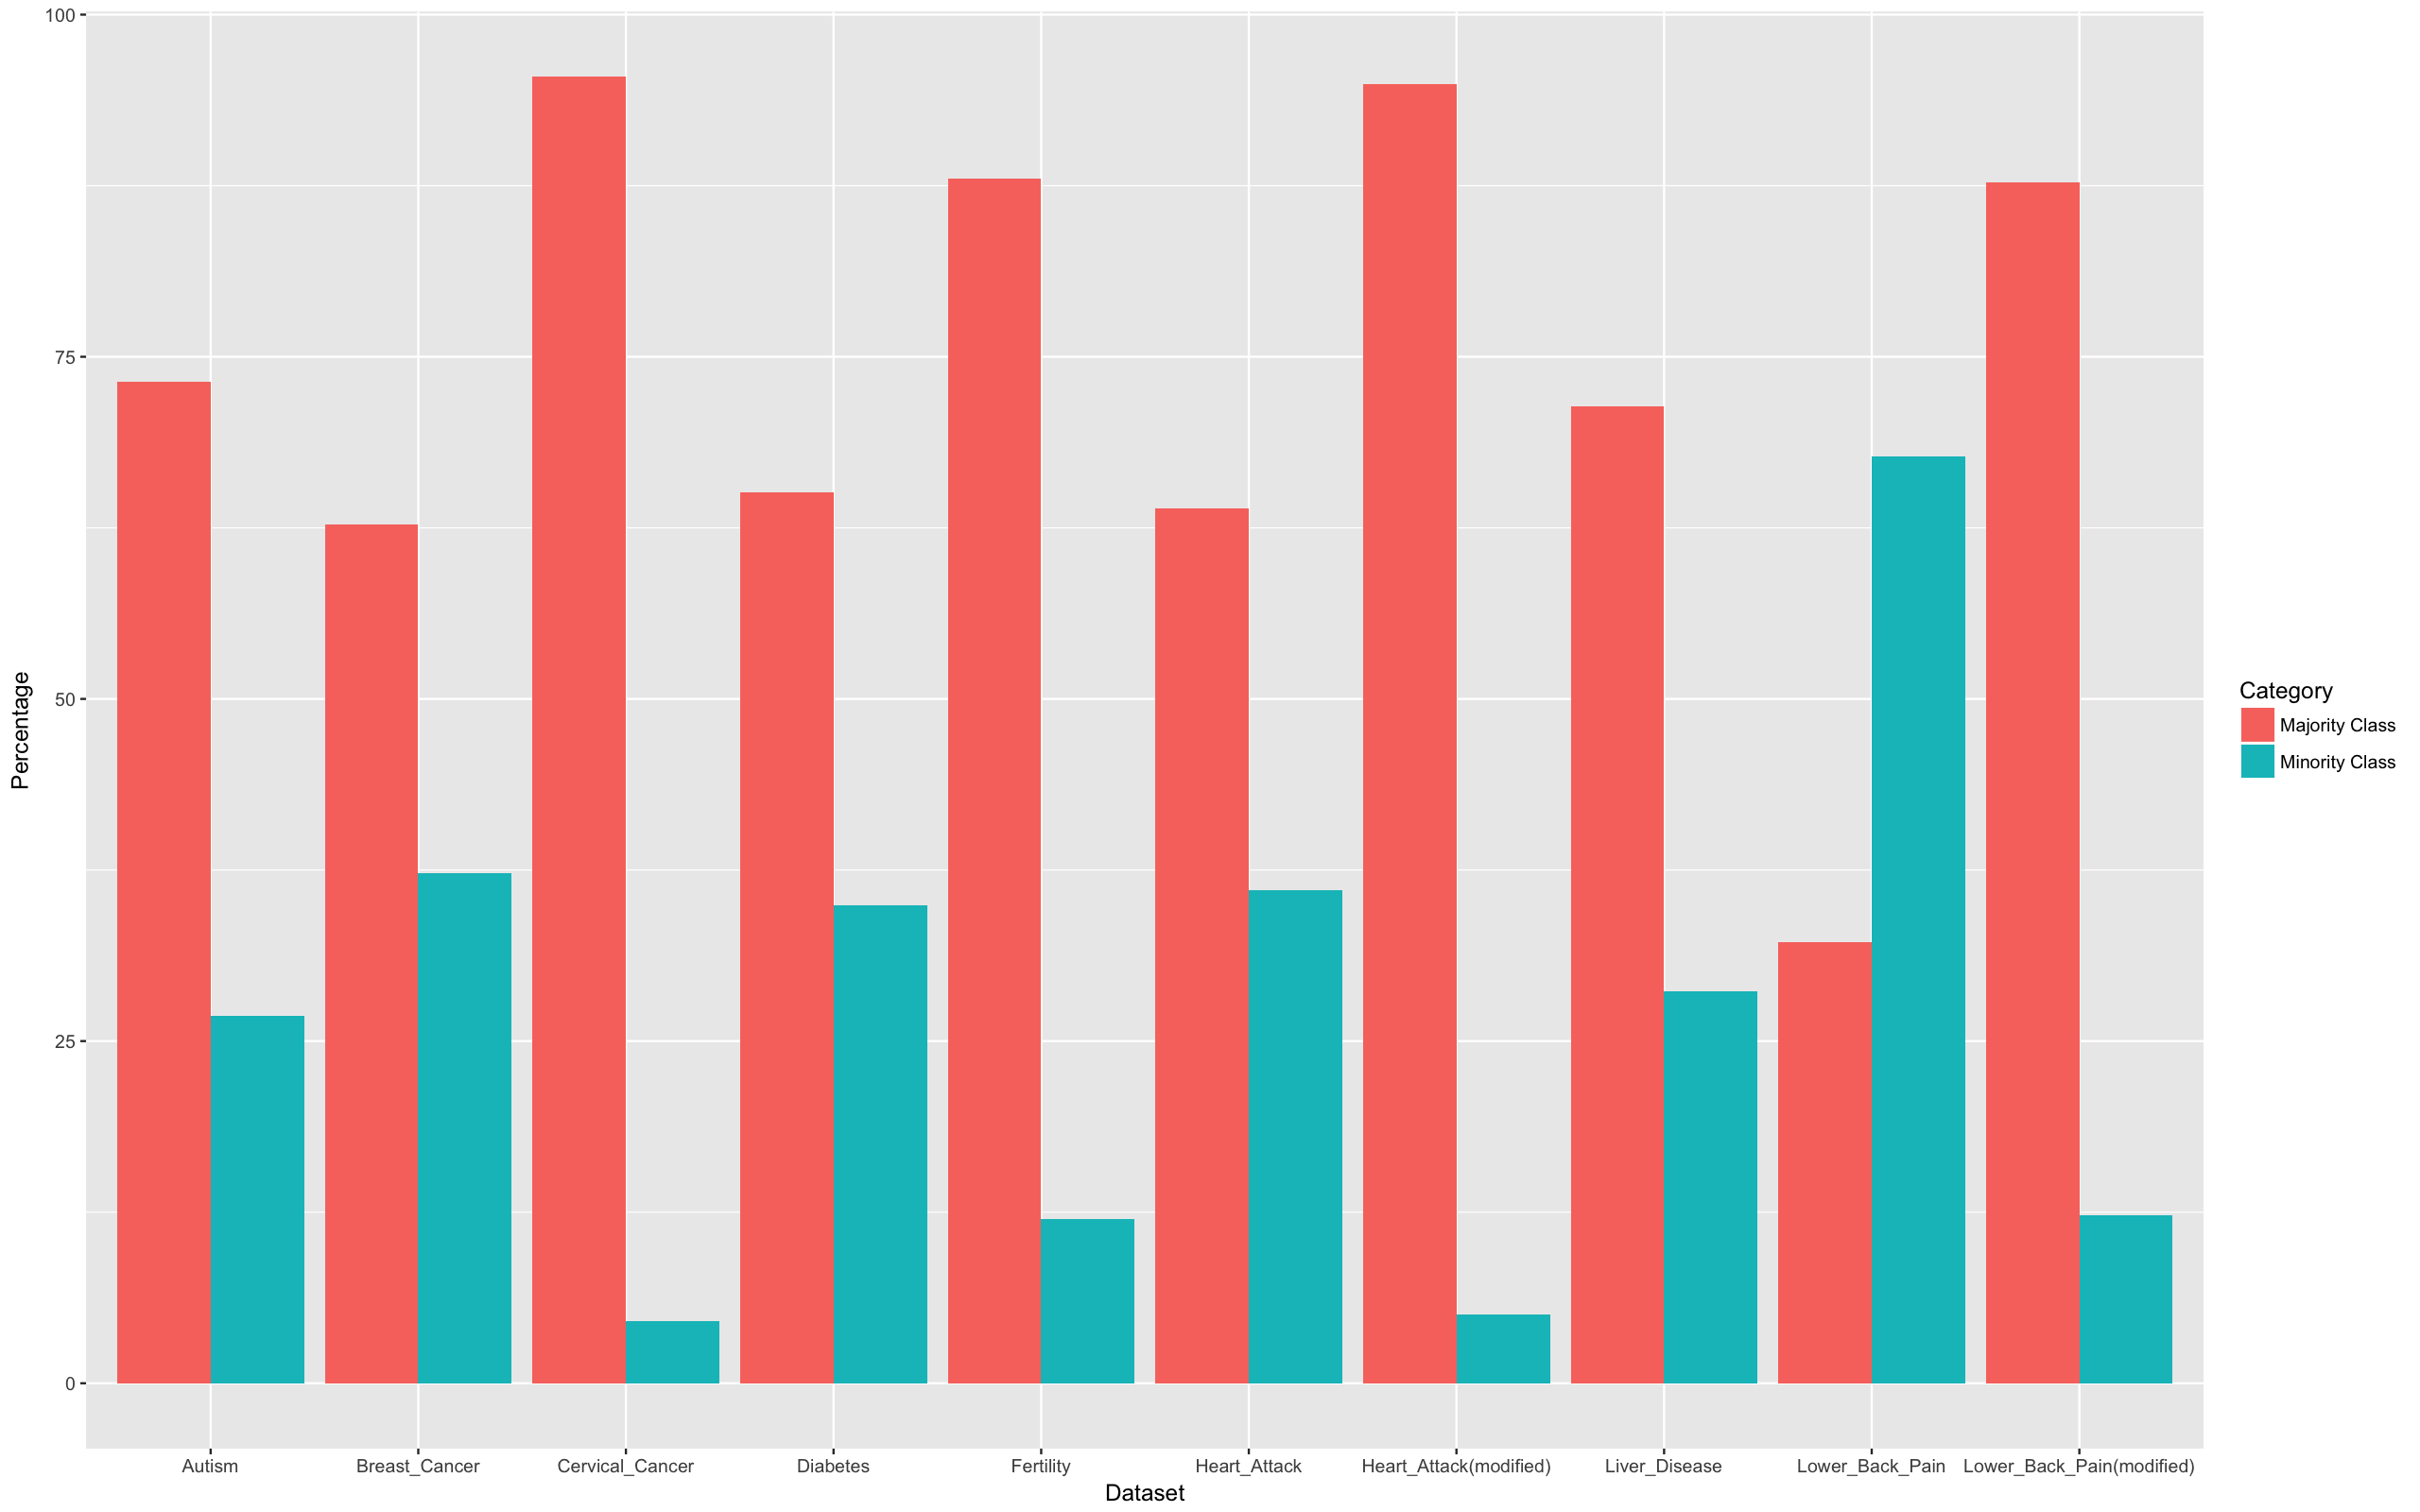
\includegraphics[width=0.9\textwidth]{ThesisTemplate/usingLatex/chapter4Images/figure4_1b.png}
    \caption{Class Distribution of the chosen datasets.\newline In all cases the majority class is the class representing healthy subjects and the minority class is the class representing affected subjects.}
    \label{fig:my_label}
\end{figure}




\section{Modelling the datasets with Random Forest}
The Random Forest algorithm was used with all the datasets. 
An R script (see linked repository, Experiment1.R and RandomForestModelling.R) was created to classify all 10 datasets and obtain a baseline of the performance that could be obtained on the dataset after pre-processing as detailed in section 4.1.
\subsubsection{Procedure and parameters}
The dataset were uploaded as a list which was iterated through by the R function randomForest(). 
The data split was 70:30 train: test and the number of trees was 128 as Oshiro and colleagues showed that setting the number of trees to higher values mostly only used more CPU but did not improve algorithm performance\citep{MayumiOshiro:ve}. Proximity and importance were both set as true.\newline
The RandomForestModelling.R script output  a data frame containing performance metrics (Accuracy, Precision, Sensitivity and F1 score) of the algorithm for each dataset.\newline
Parameters pertaining to the randomForest() function were modifiable through the randomForestModelling function created in the script so that different situations could be easily modelled.


\section{Modelling the datasets with data-level solutions applied}
\subsection{Under-sampling of the majority class}
An R script was created to fit Random Forest to the datasets after under sampling the majority class in an attempt to address the class imbalance. 
Under-sampling means that a proportion of the majority class will be discarded at random with a view to create a more balanced dataset(The diagram in figure 4.2 illustrate under-sampling).\newline
Under-sampling leads to loss of data and though it is expected some metrics will improve, it is also likely that others will worsen; for example precision may increase but sensitivity may decrease.\newline

\begin{figure}[!htbp]
    \centering
    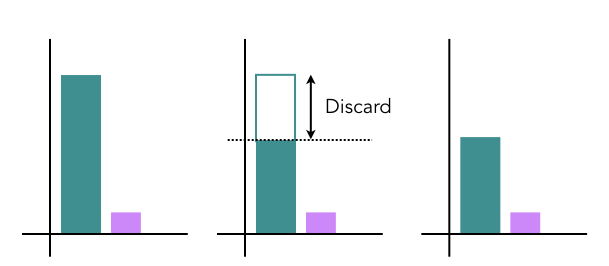
\includegraphics[width=0.9\textwidth]{ThesisTemplate/usingLatex/chapter4Images/Figure2001.png}
    \caption{Under-sampling the majority class. A proportion of the data in the majority class is discarded resulting in more balanced dataset}
    \label{fig:my_label}
\end{figure}


A function to retain different proportion of each class to include in the experiment was devised. Several different percentages of majority class data were tested, while always retained 100 \% of the minority class.
The proportion of each class to include for input in the Random Forest algorithm can be changed as parameters of the function.
The default value for the function was 40\% of the majority class and 100\% of the minority class retained.\newline
Three different values were tested for under-sampling of the majority class:
\begin{itemize}
    \item 40\% of majority class retained
    \item 60\% of majority class retained
    \item 75\% of majority class retained
\end{itemize}

In all cases 100\% of the minority class was retained.\newline
The modified datasets were then fed through the RandomForestModelling script and the accuracy, sensitivity precision and F1 score were recorded to evaluate the effects of the under-sampling on the performance of the algorithm for each dataset.\newline



\subsection{Oversampling of the minority class}
In order to address the class imbalance, this experiment examined the effect of oversampling the minority class. To achieve oversampling, the Synthetic Minority Oversampling Technique or SMOTE \citep{Chawla:2002ty} was applied. \newline 
This technique creates new data points for the minority class from existing data by considering a number of the closest neigbouring points to each existing data points.Figure 4.3 illustrates the over-sampling of minority class by SMOTE. The DMwR package in R contains the smote() function which implements the SMOTE algorithm in R \citep{Anonymous:bPzTqa7x}.\newline

\begin{figure}[!htbp]
    \centering
    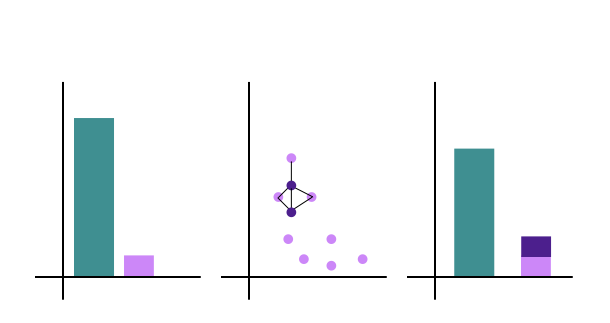
\includegraphics[width=0.9\textwidth]{ThesisTemplate/usingLatex/chapter4Images/Figure2002.png}
    \caption{Over-sampling the minority class. New data points for the minority class are created from existing cases, resulting in a more balanced dataset}
    \label{fig:my_label}
\end{figure}


The number of existing neighbouring data points to be considered is the \textbf{parameter k} of the smote() function and can be set experimentally to give best results.\newline
The \textbf{k value} is set by default at k=5. However, if k exceeds the number of minority class observations in the training set, an error will occur as there will not be enough points to create the new data point.\newline
Two other parameters need to be set for the function: 
\begin{itemize}
    \item \textbf{perc.over}to set the number of extra cases from the minority class are generated. This is typically a value above 100 so that for each case of the minority class in the original dataset, perc.over/100 new cases will be created.
    \item \textbf{perc.under} controls the number of proportion of cases of the majority class that will be randomly selected for the final balanced dataset. This is calculated based on the the number of newly created minority class cases. 
\end{itemize}

The smote() function is applied only to the training set, in order to train the model,  not the testing set.\newline
The k value used when applying smote to the non modified datasets was k=4.\newline()
The smote() function was applied to the modified heart attack dataset and low back pain dataset with separate parameters from the other datasets, as the generally lower number of observation existing in the sample meant that too few majority class observations were retained. The parameters for these datasets were 200, 600 and k= 4.
Finally the fertility datasets consists of a low number of observation and smote() was also applied with separate parameters so as to retain a larger number of majority class observation (200, 600 k=4).



\section{Conclusions}
Three different sets of experiments were carried on all eight datasets with a view to compare the resulting accuracy, precision, sensitivity and F1 score for each dataset in each situation. The results will be plotted and discussed in chapter 5.


